% =====================================================================
%  Presentación del Trabajo de Grado
%  "Efectos de la densidad de energía gravitacional sobre la velocidad
%   de la luz: verificación experimental de la Hipótesis de Céspedes-Curé"
%  María Laura Rojas González, Universidad Simón Bolívar, 2026
%
%  Estilo y paleta inspirados en las diapositivas del Coloquio
%  Latinoamericano de Energía y Materia Oscura (U. de Carabobo, 2025).
%
%  Compilar con pdflatex (dos pasadas para el total de páginas).
%  Este archivo vive en la subcarpeta  libro/presentacion/  y toma las
%  figuras originales de la tesis desde la carpeta  libro/  (ver \graphicspath).
%  Opcional: colocar el logo de la USB como  logo-usb.png  en esta carpeta.
% =====================================================================
\documentclass[10pt,aspectratio=43,xcolor={table}]{beamer}

\usepackage[utf8]{inputenc}
\usepackage[T1]{fontenc}
\IfFileExists{lmodern.sty}{\usepackage{lmodern}}{}
\usepackage[spanish,es-noshorthands,es-nodecimaldot]{babel}
\usepackage{amsmath,amssymb}
\usepackage{graphicx}
\usepackage{booktabs}
\usepackage{array}
\usepackage{tikz}
\usetikzlibrary{shadows,calc,positioning}
\usepackage[siunitx,american]{circuitikz}
\usepackage{etoolbox}
\usepackage{ragged2e}

% Fuente tipo Calibri (como en el coloquio) si está disponible
\IfFileExists{carlito.sty}{\usepackage[sfdefault,lf]{carlito}}{}

\graphicspath{{../}{./}{./figuras/}}

% ---------------------------------------------------------------------
%  Paleta del coloquio
% ---------------------------------------------------------------------
\definecolor{verde}{HTML}{22A884}     % verde principal
\definecolor{morado}{HTML}{440154}    % morado oscuro (tablas, numeración)
\definecolor{lila}{HTML}{D9CCDC}      % filas de tablas
\definecolor{magenta}{HTML}{CC33CC}   % citas y cifras destacadas
\definecolor{amarillo}{HTML}{FDF291}  % resaltados
\definecolor{grisborde}{HTML}{DEDEDE} % marco de portadillas
\definecolor{marron}{HTML}{7F6363}    % etiquetas de ecuaciones
\definecolor{tinta}{HTML}{1A1A1A}

\setbeamercolor{normal text}{fg=tinta}
\setbeamercolor{structure}{fg=morado}
\setbeamercolor{itemize item}{fg=verde}
\setbeamercolor{itemize subitem}{fg=morado}
\setbeamercolor{enumerate item}{fg=morado}
\setbeamertemplate{itemize item}{\raisebox{0.15ex}{\color{verde}\small$\bullet$}}
\setbeamertemplate{itemize subitem}{\raisebox{0.15ex}{\color{morado}\scriptsize$\blacktriangleright$}}
\setbeamertemplate{enumerate item}{\color{morado}\insertenumlabel.}
\setbeamertemplate{navigation symbols}{}
\setbeamertemplate{footline}{}
\setbeamertemplate{headline}{}
\setbeamersize{text margin left=10mm,text margin right=10mm}

\newcommand{\cita}[1]{{\color{magenta}\scriptsize #1}}
\newcommand{\dest}[1]{{\color{magenta}#1}}
\newcommand{\etq}[1]{{\color{marron}#1}}

% ---------------------------------------------------------------------
%  Imagen con respaldo (si falta el archivo se dibuja un recuadro)
% ---------------------------------------------------------------------
\newcommand{\img}[2]{%
  \IfFileExists{../#2}{\includegraphics[#1]{#2}}{%
  \IfFileExists{#2}{\includegraphics[#1]{#2}}{%
  \IfFileExists{figuras/#2}{\includegraphics[#1]{#2}}{%
    \fbox{\parbox[c][18mm][c]{30mm}{\centering\tiny\color{gray}#2}}}}}}

% ---------------------------------------------------------------------
%  Tablas con el estilo del coloquio
% ---------------------------------------------------------------------
\newcommand{\cabecera}{\rowcolor{morado}}
\newcommand{\thc}[1]{{\color{white}\bfseries #1}}
\newcommand{\filalila}{\rowcolor{lila}}

% ---------------------------------------------------------------------
%  Diseños de fondo (equivalentes a los layouts del PowerPoint)
%     banda   : título arriba + banda verde + tarjeta con sombra
%     barra   : barra verde vertical a la izquierda + tarjeta
%     foto    : franja verde inferior + tarjeta a la derecha
%     bloque  : bloque verde a la derecha + tarjeta grande
%     limpio  : sólo numeración
% ---------------------------------------------------------------------
\newcommand{\curlayout}{banda}
\newcommand{\layout}[1]{\renewcommand{\curlayout}{#1}}

\tikzset{tarjeta/.style={fill=white,draw=none,
  drop shadow={opacity=0.28,shadow xshift=0.5mm,shadow yshift=-0.7mm,fill=black!60}}}

% coordenadas en mm desde la esquina superior izquierda
\newcommand{\Pt}[2]{($(current page.north west)+(#1mm,-#2mm)$)}

\newcommand{\numeracion}{%
  \node[anchor=north east,text=morado,font=\footnotesize] at \Pt{125}{2.2}
    {\insertframenumber/\inserttotalframenumber};}

\setbeamertemplate{background}{%
\begin{tikzpicture}[remember picture,overlay]
  \ifdefstring{\curlayout}{banda}{%
    \fill[verde] \Pt{0}{28} rectangle \Pt{120}{31};
    \fill[verde] \Pt{121}{28} rectangle \Pt{122.6}{39};
    \fill[tarjeta] \Pt{0}{31} rectangle \Pt{119.6}{89};
  }{}%
  \ifdefstring{\curlayout}{barra}{%
    \fill[verde] \Pt{3.5}{0} rectangle \Pt{9}{12.8};
    \fill[verde] \Pt{3.5}{12.8} rectangle \Pt{6}{78};
    \fill[verde] \Pt{3.5}{79.5} rectangle \Pt{6}{81.8};
    \fill[tarjeta] \Pt{6}{12.8} rectangle \Pt{122.6}{89};
  }{}%
  \ifdefstring{\curlayout}{foto}{%
    \fill[verde] \Pt{1}{62} rectangle \Pt{3.5}{91};
    \fill[verde] \Pt{4.5}{62} rectangle \Pt{128}{91};
    \fill[tarjeta] \Pt{54}{9.6} rectangle \Pt{122}{87.7};
  }{}%
  \ifdefstring{\curlayout}{bloque}{%
    \fill[verde] \Pt{78}{0} rectangle \Pt{128}{96};
    \fill[verde] \Pt{0}{25.6} rectangle \Pt{1.6}{70};
    \fill[verde] \Pt{2.6}{25.6} rectangle \Pt{4.1}{70};
    \fill[tarjeta] \Pt{4.1}{12} rectangle \Pt{120.3}{85};
  }{}%
  \numeracion
\end{tikzpicture}}

% Títulos de cada diseño
\setbeamertemplate{frametitle}{%
  \ifdefstring{\curlayout}{banda}{%
    \begin{tikzpicture}[remember picture,overlay]
      \node[anchor=base west,font=\fontsize{24}{26}\selectfont,text=black]
        at \Pt{10}{21} {\insertframetitle};
      \ifx\insertframesubtitle\empty\else
      \node[anchor=north west,text width=110mm,font=\scriptsize,text=magenta,align=left]
        at \Pt{10}{22} {\insertframesubtitle};\fi
    \end{tikzpicture}\vspace*{24mm}}{}%
  \ifdefstring{\curlayout}{barra}{%
    \begin{tikzpicture}[remember picture,overlay]
      \node[anchor=base west,font=\fontsize{24}{26}\selectfont,text=black]
        at \Pt{11}{10} {\insertframetitle};
    \end{tikzpicture}\vspace*{9mm}}{}%
  \ifdefstring{\curlayout}{foto}{%
    \begin{tikzpicture}[remember picture,overlay]
      \node[anchor=north west,text width=44mm,align=left,
        font=\fontsize{17}{19}\selectfont\bfseries,text=morado]
        at \Pt{7}{10} {\insertframetitle};
    \end{tikzpicture}}{}%
  \ifdefstring{\curlayout}{bloque}{%
    \begin{tikzpicture}[remember picture,overlay]
      \node[anchor=base west,font=\fontsize{20}{22}\selectfont,text=morado]
        at \Pt{10}{9} {\insertframetitle};
    \end{tikzpicture}\vspace*{9mm}}{}%
  \ifdefstring{\curlayout}{limpio}{%
    \begin{tikzpicture}[remember picture,overlay]
      \node[anchor=base west,font=\fontsize{20}{22}\selectfont,text=morado]
        at \Pt{10}{10} {\insertframetitle};
    \end{tikzpicture}\vspace*{8mm}}{}%
}

% Contenido a la derecha en el diseño "foto" (dentro de la tarjeta)
\newcommand{\derecha}[1]{%
  \begin{tikzpicture}[remember picture,overlay]
    \node[anchor=center,text width=62mm,align=center] at \Pt{88}{48.6} {#1};
  \end{tikzpicture}}

% Texto de la columna izquierda en el diseño "foto"
\newenvironment{izquierda}[1][10mm]{%
  \vspace*{#1}\hspace*{-3mm}\begin{minipage}[t]{43mm}\footnotesize\raggedright}{\end{minipage}}

% ---------------------------------------------------------------------
%  Portadilla de sección
% ---------------------------------------------------------------------
\newcommand{\seccion}[1]{%
{\setbeamertemplate{background}{%
\begin{tikzpicture}[remember picture,overlay]
  \draw[grisborde,line width=3.4mm] \Pt{5.2}{6.2} rectangle \Pt{122.6}{89.5};
  \fill[white] \Pt{88.2}{92} -- \Pt{126}{92} -- \Pt{126}{44} -- cycle;
  \fill[verde] \Pt{90.2}{91.5} -- \Pt{124.4}{91.5} -- \Pt{124.4}{46.7} -- cycle;
  \draw[black,line width=0.4pt] \Pt{79}{26} -- \Pt{79}{71};
  \node[anchor=east,align=right,text width=66mm,
        font=\fontsize{30}{36}\selectfont,text=black] at \Pt{73}{48.5} {\lefthyphenmin=64\righthyphenmin=64 #1};
  \numeracion
\end{tikzpicture}}
\begin{frame}[plain]\end{frame}}}

% =====================================================================
\title{Efectos de la densidad de energía gravitacional sobre la velocidad de la luz}
\subtitle{Verificación experimental de la Hipótesis de Céspedes-Curé}
\author{María Laura Rojas González}
\date{Octubre de 2026}

\begin{document}

% ---------------------------------------------------------------------
%  PORTADA
% ---------------------------------------------------------------------
{\setbeamertemplate{background}{%
\begin{tikzpicture}[remember picture,overlay]
  \draw[black!75,line width=0.6pt] \Pt{6.8}{8.7} rectangle \Pt{121.2}{87};
  \fill[verde] \Pt{93.8}{91.5} -- \Pt{124.4}{91.5} -- \Pt{124.4}{46.7} -- cycle;
  \node at \Pt{64}{17.5} {\IfFileExists{logo-usb.png}{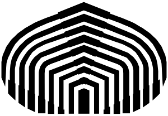
\includegraphics[height=11mm]{logo-usb.png}}{}};
  \node[align=center,text width=104mm,font=\fontsize{19}{22}\selectfont] at \Pt{64}{40}
    {Efectos de la densidad de energía gravitacional sobre la velocidad de la luz:\\[1mm]
     {\fontsize{16}{19}\selectfont Verificación experimental de la hipótesis de Céspedes-Curé}};
  \node[anchor=north west,align=left,font=\normalsize] at \Pt{15}{62}
    {María Laura Rojas González\\[0.6mm]
     {\small Tutor: Dr. Eduardo Greaves}\\[1mm]
     {\footnotesize\color{black!65}Trabajo de grado para optar al título de Licenciada en Física}\\[0.3mm]
     {\footnotesize\color{black!65}Universidad Simón Bolívar, Coordinación de Física}};
  \node[font=\scriptsize,text=magenta] at \Pt{64}{89.8}
    {Sartenejas, octubre de 2026};
  \numeracion
\end{tikzpicture}}
\begin{frame}[plain]\end{frame}}

% ---------------------------------------------------------------------
\layout{banda}
\begin{frame}{Contenido}
\vspace{2mm}
\begin{enumerate}\setlength{\itemsep}{2.2mm}
  \item Hipótesis de Céspedes-Curé (HCC)
  \item Antecedentes y justificación: Pioneer, Flyby y datos históricos de $c$
  \item Experimento I: medición directa de la velocidad de la luz
  \item Experimento II: medición indirecta con un circuito resonante
  \item Propuestas de mejora y experimentos propuestos
  \item Conclusiones
\end{enumerate}
\end{frame}

% ---------------------------------------------------------------------
\begin{frame}{Introducción}
\small
\begin{itemize}\setlength{\itemsep}{1.6mm}
  \item La Relatividad Especial (1905) postula que la luz viaja a velocidad constante en el vacío.
        Sobre ese postulado descansan el efecto Doppler astronómico y la definición actual del metro.
  \item Céspedes-Curé (2002) propone que el espacio no está vacío: es un \textbf{medio energético}
        en el que $c$ depende de la densidad de energía local.
  \item Con esta idea se han explicado la \dest{Pioneer Anomaly} (2007) y la \dest{Flyby Anomaly} (2020).
  \item Entre la USB, el Teleférico de Caracas y Carmen de Urea la HCC predice diferencias en $c$ sólo
        a partir de la \textbf{novena cifra significativa}: se necesita una precisión mejor que $\pm1$~m/s.
\end{itemize}
\vspace{1mm}
\begin{tikzpicture}
\node[fill=amarillo,rounded corners=3mm,text width=94mm,inner sep=2.5mm,font=\small]
{\textbf{Hipótesis del trabajo:} si la densidad de energía gravitacional altera las propiedades
 del vacío, la velocidad de un haz láser modulado y la frecuencia de resonancia de un circuito RLC
 deben cambiar de forma medible con la altitud.};
\end{tikzpicture}
\end{frame}

% =====================================================================
\seccion{Hipótesis de Céspedes-Curé}
% =====================================================================

\layout{banda}
\begin{frame}{Densidad de Energía}
\vspace{1mm}
Es la cantidad de energía por unidad de volumen almacenada en un espacio debido a un campo.
\vspace{2mm}
\begin{align*}
 &\etq{\text{Campo Eléctrico}}\quad \rho_e=\frac{E^2}{8\pi K_e}\;\etq{=}\;\frac{K_eQ^2}{8\pi r^4}\\[0.5mm]
 &\etq{\text{Campo Magnético}}\quad \rho_m=\frac{B^2}{2\mu_0}\\[0.5mm]
 &\etq{\text{Campo Gravitacional}}\quad \rho_g=\frac{\etq{g}^2}{8\pi G}\;\etq{=}\;\frac{GM^2}{8\pi r^4}
\end{align*}
\vspace{1mm}
En un laboratorio terrestre la densidad total incluye las estrellas lejanas $\rho^*$:
\[
\rho=\rho^*+\frac{GM^2}{8\pi r^4}+\frac{1}{2}\,\mathbf{E}\cdot\mathbf{D}+\frac{1}{2}\,\mathbf{B}\cdot\mathbf{H}
\]
\cita{Céspedes-Curé, J.: Einstein on Trial or Metaphysical Principles of Natural Philosophy, 2002.}
\end{frame}

% ---------------------------------------------------------------------
\layout{bloque}
\begin{frame}
\begin{columns}[T]
\begin{column}{0.60\textwidth}
\vspace{4mm}
{\fontsize{30}{34}\selectfont Hipótesis de\\[1mm] Céspedes-Curé}
\vspace{6mm}

\small A partir de las ecuaciones de Maxwell, la densidad de energía obedece una ecuación de
D'Alembert inhomogénea:
\[
\nabla^2\rho-c^{-2}\frac{\partial^2\rho}{\partial t^2}=\nabla\cdot\mathbf{T}
\]
las ondas electromagnéticas son ondas de densidad de energía.
\end{column}
\begin{column}{0.36\textwidth}
\vspace{18mm}
\centering
\begin{tikzpicture}
\node[fill=white,draw=verde,line width=1pt,inner sep=4mm,font=\fontsize{26}{30}\selectfont]
  {$c=\dfrac{k}{\sqrt{\etq{\rho}}}$};
\end{tikzpicture}

\vspace{3mm}
{\scriptsize $k$: constante\\ $\rho$: densidad de energía total}
\end{column}
\end{columns}
\end{frame}

% =====================================================================
\seccion{Antecedentes\\ y justificación}
% =====================================================================

\layout{barra}
\begin{frame}{Pioneer Anomaly}
\begin{columns}[T]
\begin{column}{0.56\textwidth}
\small\justifying
Las sondas Pioneer 10 y 11 mostraron, a más de 20~UA, una aceleración anómala constante hacia el Sol
de $\sim 8\times10^{-8}$~cm/s$^2$ que ninguna causa sistemática logró justificar.

\vspace{2mm}
La velocidad se mide por efecto Doppler suponiendo $c$ constante. Greaves$^*$ propone que el cambio de
$c$ debido a la HCC explica la anomalía:
\end{column}
\begin{column}{0.40\textwidth}
\vspace{2mm}
\[
n'=\frac{\sqrt{\rho^*+\rho_{S,\text{lejos}}+\rho_{E,\text{lejos}}}}{\sqrt{\rho^*+\rho_{S,1\text{UA}}+\rho_E}}
\]
\[
a=G\left(\frac{M_S}{r_S^2}-\frac{M_E}{r_E^2}\right)(1-n')
\]
\[
n'_{20\,\text{UA}}=0.9999735679
\]
\end{column}
\end{columns}
\vfill
\cita{$^*$Greaves, E. D.: NASA's astonishing evidence that c is not constant: The pioneer anomaly, 2007. https://arxiv.org/abs/physics/0701130.}
\end{frame}

% ---------------------------------------------------------------------
\begin{frame}{Pioneer Anomaly}
\small
Con el índice de refracción necesario para explicar la aceleración observada se calcula la
densidad de energía gravitacional de las estrellas lejanas $\rho^*$.

\vspace{2mm}
Valor que difiere en \textbf{menos del 1\%} del calculado por Céspedes-Curé con un método
totalmente distinto (deflexión de la luz en eclipses, ley de Merat).

\vspace{5mm}
\centering
\renewcommand{\arraystretch}{1.6}
\begin{tabular}{p{45mm}p{45mm}}
\cabecera \thc{Calculado por Greaves a partir de Pioneer Anomaly} & \thc{Calculado por Céspedes-Curé a partir de los eclipses}\\
\filalila \rule{0pt}{8mm}\large $1{,}0838\times10^{15}$ J/m$^3$ & \large $1{,}094291\times10^{15}$ J/m$^3$\\
\end{tabular}
\vfill
\raggedright\cita{Greaves, E. D.: NASA's astonishing evidence that c is not constant: The pioneer anomaly, 2007.}
\end{frame}

% ---------------------------------------------------------------------
\layout{banda}
\begin{frame}{Flyby Anomaly}{Greaves, Bracho y Mikoss: A Solution to the Flyby Anomaly Riddle. Progress in Physics, 16:49--57, 2020.}
\begin{columns}[T]
\begin{column}{0.47\textwidth}
\begin{tikzpicture}
\node[fill=amarillo,rounded corners=3mm,text width=50mm,inner sep=2mm,font=\small,align=justify]
{La maniobra de asistencia gravitatoria usa un cuerpo masivo para cambiar la trayectoria de las sondas.};
\end{tikzpicture}

\vspace{2mm}
\small\justifying
En Galileo, NEAR, Cassini, Rosetta y MESSENGER se detectó un cambio anormal de energía cinética en
sobrevuelos cercanos a la Tierra: aumento, reducción o ninguna anomalía.
\end{column}
\begin{column}{0.51\textwidth}
\footnotesize
La anomalía depende de los puntos de entrada ($-$) y salida ($+$):
\[
V_{anom}=V_\infty\left(\sqrt{\frac{\rho}{\rho'_+}}-\sqrt{\frac{\rho}{\rho'_-}}\right)
\]
\vspace{-2mm}
\[
\rho'_\pm=\rho^*+\frac{GM_E}{(r_E^\pm)^2}+\frac{GM_S}{(r_S^\pm)^2}
\]
\begin{itemize}\setlength{\itemsep}{0.5mm}
\item $r_S^+=r_S^-$, $r_E^+=r_E^-$: sin anomalía.
\item $r_S^+\neq r_S^-$, $r_E^+=r_E^-$: anomalía muy pequeña.
\item $r_S^+\neq r_S^-$, $r_E^+\neq r_E^-$: anomalía detectable.
\end{itemize}
\end{column}
\end{columns}
\end{frame}

% ---------------------------------------------------------------------
\begin{frame}{Flyby Anomaly}{Greaves, Bracho y Mikoss: A Solution to the Flyby Anomaly Riddle. Progress in Physics, 16:49--57, 2020.}
\small
La HCC predice la anomalía de sobrevuelo de Galileo I (1990) y NEAR (1998) con diferencias de
alrededor del \textbf{0,5\%}.

\vspace{3mm}
\centering\scriptsize
\renewcommand{\arraystretch}{1.3}
\setlength{\tabcolsep}{2.5pt}
\resizebox{\linewidth}{!}{\begin{tabular}{lcccc}
\toprule
 & \multicolumn{2}{c}{Galileo 1} & \multicolumn{2}{c}{NEAR}\\
 & Entrada & Salida & Entrada & Salida\\
\midrule
Distancia al Sol (m)   & $1.502803\times10^{11}$ & $1.502831\times10^{11}$ & $1.495630\times10^{11}$ & $1.495950\times10^{11}$\\
Distancia a la Tierra (m) & $1.7651\times10^{7}$ & $1.4864\times10^{7}$ & $7.2000\times10^{7}$ & $1.2200\times10^{7}$\\
Velocidad (m/s) & \multicolumn{2}{c}{8949} & \multicolumn{2}{c}{6851}\\
Anomalía medida (mm/s) & \multicolumn{2}{c}{3.930} & \multicolumn{2}{c}{13.46}\\
Anomalía calculada (mm/s) & \multicolumn{2}{c}{3.944} & \multicolumn{2}{c}{13.38}\\
\rowcolor{lila} Diferencia (\%) & \multicolumn{2}{c}{$+0.40$} & \multicolumn{2}{c}{$-0.57$}\\
\bottomrule
\end{tabular}}
\end{frame}

% ---------------------------------------------------------------------
\begin{frame}{Datos históricos}{Ramdani, F.: Gravity Constraints on the Measurements of the Speed of Light. Int. J. of Astronomy and Astrophysics, 9:265--273, 2019.}
\begin{columns}[T]
\begin{column}{0.50\textwidth}
\small\justifying
Las medidas históricas de $c$ discrepan a partir de la séptima cifra significativa. Ramdani halla una
\textbf{relación lineal de pendiente negativa} entre $c$ medida y la gravedad local del laboratorio.

\vspace{2mm}
Aplicando la HCC en un punto $i$ de la Tierra con gravedad $g_i$:
\[
c_i=c_E\,\frac{\sqrt{\rho^*+\rho_S+\rho_E}}{\sqrt{\rho^*+\rho_S+\dfrac{g_i^2}{8\pi G}}}
\]
{\scriptsize $\rho^*=1.0838\times10^{15}$, $\rho_S=2.097\times10^{4}$, $\rho_E=5.726\times10^{10}$ J/m$^3$}
\end{column}
\begin{column}{0.48\textwidth}
\centering\scriptsize
\renewcommand{\arraystretch}{1.05}
\setlength{\tabcolsep}{3pt}
\begin{tabular}{lccc}
\cabecera \thc{Año} & \thc{$c$ (m/s)} & \thc{Error} & \thc{$g$ (m/s$^2$)}\\
1953 & 299\,792\,400 & 110 & 9.811856\\
\filalila 1953$^\dagger$ & 299\,792\,200 & 130 & 9.818074\\
1955 & 299\,792\,400 & 400 & 9.816501\\
\filalila 1967 & 299\,792\,500 & 50 & 9.810565\\
1971 & 299\,792\,375 & 60 & 9.819047\\
\filalila 1972 & 299\,792\,460 & 6 & 9.794161\\
1974 & 299\,792\,459 & 0.8 & 9.811856\\
\filalila 1978 & 299\,792\,458.8 & 0.2 & 9.811856\\
1979 & 299\,792\,458.1 & 1.9 & 9.80616\\
\filalila 1983 & 299\,792\,458.6 & 0.3 & 9.800849\\
\end{tabular}

\vspace{1mm}
{\tiny $^\dagger$Geodímetro. 1953 a 1971: geodímetro; 1972 a 1983: láser.}
\end{column}
\end{columns}
\end{frame}

% ---------------------------------------------------------------------
\layout{limpio}
\begin{frame}
\vspace{-4mm}
\begin{columns}[T]
\begin{column}{0.55\textwidth}
\begin{tikzpicture}
\node[tarjeta,inner sep=2mm] {\small$\displaystyle c_i=c_E\,\frac{\sqrt{\rho^*+\rho_S+\rho_E}}{\sqrt{\rho^*+\rho_S+\frac{g_i^2}{8\pi G}}}$};
\end{tikzpicture}

\vspace{6mm}
\small Valores de $c$ históricos vs gravedad local, junto con la línea que predice la HCC:

\vspace{1mm}
\img{width=\linewidth}{Imagen4.png}

\vspace{1mm}
{\scriptsize La mayoría de los puntos concuerdan con la predicción dentro de su error.}
\end{column}
\begin{column}{0.42\textwidth}
\begin{tikzpicture}
\node[tarjeta,inner sep=1.5mm] {\begin{tabular}{c}
\img{width=44mm}{Curva c_i vs g_i.png}\\[1mm]
\img{width=44mm}{curva c_i vs g_i zoom.png}\end{tabular}};
\end{tikzpicture}
\end{column}
\end{columns}
\begin{tikzpicture}[remember picture,overlay]
\fill[verde] \Pt{0}{14} rectangle \Pt{1.6}{24};
\fill[verde] \Pt{2.6}{14} rectangle \Pt{4.1}{24};
\fill[verde] \Pt{9}{90} rectangle \Pt{119}{91.2};
\end{tikzpicture}
\end{frame}

% ---------------------------------------------------------------------
{\setbeamertemplate{background}{%
\begin{tikzpicture}[remember picture,overlay]
  \fill[verde] \Pt{0}{0} rectangle \Pt{128}{62};
  \fill[tarjeta] \Pt{6.3}{7.8} rectangle \Pt{121.7}{72};
  \fill[verde] \Pt{6.3}{88} rectangle \Pt{121.7}{89.6};
  \numeracion
\end{tikzpicture}}
\begin{frame}[plain]
\vspace*{2mm}
\centering
{\large\color{morado} Resultados esperados en las tres localidades}

\vspace{3mm}
\renewcommand{\arraystretch}{1.7}
\small
\begin{tabular}{>{\columncolor{morado}\color{white}\bfseries}l p{27mm}p{27mm}p{27mm}}
 & \textbf{Carmen de Urea} & \textbf{USB} & \textbf{Teleférico}\\
Altura & 20.36 m & 1176 m & 2119 m\\
\filalila \cellcolor{morado}Gravedad m/s$^2$ & 9.7825124 & 9.77967685 & 9.777794\\
Velocidad m/s & 29979247\dest{1.69} & 29979247\dest{3.97} & 29979247\dest{5.47}\\
\filalila \cellcolor{morado}$f_0$ Hz & 103318.57\dest{0664} & 103318.57\dest{1449} & 103318.57\dest{1966}\\
\end{tabular}

\vspace{4mm}
\begin{minipage}{108mm}\footnotesize
Los valores de $c$ difieren a partir de la \textbf{novena cifra significativa}. $f_0$: frecuencia de
resonancia de un mismo circuito RLC con $k_0=0.002165397$ m$^{-1}$ ($f_0/f_{\text{Carmen}}=1.000000013$ en el Teleférico).
\end{minipage}

\vfill
{\scriptsize\color{white!20!black} Gravedad: comunicación personal de la Dra. Nuris Orihuela (UCV).}
\end{frame}}

% ---------------------------------------------------------------------
\layout{banda}
\begin{frame}{Implicaciones de la HCC}
\begin{columns}[T]
\begin{column}{0.56\textwidth}
\footnotesize
\begin{itemize}\setlength{\itemsep}{1mm}
\item \textbf{Curvas de rotación planas:} $\rho_g$ es mayor en el centro galáctico, $c$ crece hacia los
bordes y el Doppler sobreestima la velocidad de las estrellas. No haría falta la materia oscura.
\item \textbf{Expansión acelerada:} $\rho_g$ decrece hacia los límites, $n'$ disminuye y se
sobreestiman las velocidades de recesión.
\item \textbf{Deflexión de la luz en eclipses:} refracción por el índice $n(r)$ cerca del Sol.
\item \textbf{Agujeros negros:} $\rho_g$ tan grande que $c$ se hace muy pequeña.
\end{itemize}
\end{column}
\begin{column}{0.42\textwidth}
\vspace{2mm}
\centering
\img{width=\linewidth}{CurvaPlanaGalaxias.png}

{\tiny Curvas de rotación de galaxias espirales (Carroll y Ostlie).}
\end{column}
\end{columns}
\end{frame}

% =====================================================================
\seccion{Experimento I:\\ medición\\ directa}
% =====================================================================

\layout{foto}
\begin{frame}{Montaje\\experimental}
\begin{izquierda}
Un haz láser de He-Ne modulado se divide: un brazo recorre una distancia variable y el otro una fija.
El desfase crece con la diferencia de camino:
\[ \Delta x=c\,\Delta t \]
\vspace{-2mm}
\begin{itemize}\setlength{\itemsep}{0mm}\footnotesize
\item Láser He-Ne, lente, espejo, divisor de haz
\item Generador de señal modulada con fotodetectores
\item Osciloscopio Tektronix TDS 2024B
\end{itemize}
\end{izquierda}
\derecha{\img{width=58mm}{experimento_guia.png}\\[1mm]
{\tiny Esquema de la práctica de Laboratorio 3, USB.}}
\end{frame}

% ---------------------------------------------------------------------
\begin{frame}{Análisis\\de datos}
\begin{izquierda}
\begin{itemize}\setlength{\itemsep}{1mm}\footnotesize
\item Desfase medido con los cursores del osciloscopio (promedio de varias lecturas).
\item Datos digitales (.csv) ajustados con Python: FFT para la frecuencia inicial y \texttt{curve\_fit}.
\end{itemize}
\[ A\sin(\omega t+\phi)+\text{offset} \]
\[ \Delta t=2\,\frac{|\phi_2-\phi_1|}{\omega_2+\omega_1} \]
\end{izquierda}
\derecha{\img{width=48mm}{F0003TEK.png}\\[2mm]\img{width=50mm}{AjusteF0003CH2.png}}
\end{frame}

% ---------------------------------------------------------------------
\layout{barra}
\begin{frame}{Resultados}
\begin{columns}[T]
\begin{column}{0.44\textwidth}
\small
Mediciones entre 4 y 7 distancias (10 m a 30 m). Las gráficas debían ser rectas:

\vspace{2mm}
\centering\footnotesize
\renewcommand{\arraystretch}{1.35}
\begin{tabular}{cc}
\cabecera \thc{Medida} & \thc{Pendiente (m/s)}\\
n1 & $(3.1666\pm9.4493)\times10^{8}$\\
\filalila n2 & $(0.2838\pm0.5678)\times10^{8}$\\
n3 & $(-0.2135\pm0.2775)\times10^{8}$\\
\filalila n4.1, n4.2 & No aplica\\
\end{tabular}
\end{column}
\begin{column}{0.54\textwidth}
\centering
\img{width=0.49\linewidth}{n-1.png}\hfill\img{width=0.49\linewidth}{n-2.png}\\[1mm]
\img{width=0.49\linewidth}{n-3.png}

\vspace{1mm}
{\scriptsize Pendientes con incertidumbres enormes, órdenes de magnitud erróneos e incluso signo negativo.}
\end{column}
\end{columns}
\end{frame}

% ---------------------------------------------------------------------
\begin{frame}{Mejoras del método}
\begin{columns}[T]
\begin{column}{0.46\textwidth}
\small
\begin{itemize}\setlength{\itemsep}{1mm}
\item Lente de distancia focal corta con soporte fijo.
\item Todos los elementos a la misma altura.
\item De 7 a 15 puntos por medida.
\item Experimento en el pasillo: diferencias de camino de 40 m a 80 m.
\end{itemize}
\vspace{2mm}
\centering\footnotesize
\renewcommand{\arraystretch}{1.35}
\begin{tabular}{ccc}
\cabecera \thc{Medida} & \thc{Pendiente (m/s)} & \thc{Error}\\
n5.1 & $(3.0296\pm0.0556)\times10^{8}$ & \dest{1\%}\\
\filalila n5.2 & $(3.1965\pm0.0355)\times10^{8}$ & 6\%\\
\end{tabular}
\end{column}
\begin{column}{0.52\textwidth}
\centering
\img{width=0.92\linewidth}{n-5.1.png}\\[1mm]
\img{width=0.92\linewidth}{n-5.2.png}
\end{column}
\end{columns}
\end{frame}

% ---------------------------------------------------------------------
\layout{banda}
\begin{frame}{Cálculo de la precisión necesaria}
\begin{columns}[T]
\begin{column}{0.50\textwidth}
\small
Para distinguir las localidades se necesita $E_c\le1$ m/s. Con $c=\Delta x/\Delta t$:
\[
E_c=\frac{E_{\Delta x}}{\Delta t}+\frac{\Delta x}{(\Delta t)^2}E_{\Delta t}
\]
Con $\Delta t\approx200$ ns y $\Delta x\approx60$ m, repartiendo el error en fracciones $\kappa+F=1$:
\[
E_{\Delta x}\sim\kappa\cdot2\times10^{-7}\ \text{m}\qquad
E_{\Delta t}\sim F\cdot6.67\times10^{-16}\ \text{s}
\]
\end{column}
\begin{column}{0.46\textwidth}
\begin{tikzpicture}
\node[fill=amarillo,rounded corners=3mm,text width=47mm,inner sep=2.5mm,font=\small,align=left]
{Se requieren distancias con precisión de \textbf{decenas de nanómetros} y desfases de
\textbf{femtosegundos}. La cinta métrica aprecia 1 mm y el ajuste da $\sim2\times10^{-10}$ s.};
\end{tikzpicture}

\vspace{3mm}
\footnotesize Evenson (1972) obtuvo $c=299792456.2(1.1)$ m/s midiendo $f$ y $\lambda$ de un láser
estabilizado con metano, con equipos fuera de nuestro alcance.
\end{column}
\end{columns}
\end{frame}

% =====================================================================
\seccion{Experimento II:\\ circuito\\ resonante}
% =====================================================================

{\setbeamertemplate{background}{%
\begin{tikzpicture}[remember picture,overlay]
  \draw[black!75,line width=0.6pt] \Pt{6.8}{8.7} rectangle \Pt{121.2}{87};
  \fill[verde] \Pt{90.2}{91.5} -- \Pt{124.4}{91.5} -- \Pt{124.4}{46.7} -- cycle;
  \numeracion
\end{tikzpicture}}
\begin{frame}[plain]
\begin{tikzpicture}[remember picture,overlay]
\node[anchor=base west,font=\fontsize{30}{32}\selectfont] at \Pt{10}{22} {Circuitos LC};
\node[anchor=north] at \Pt{34}{30} {%
 \begin{circuitikz}[scale=0.85,transform shape]
  \draw (0,0) to[sV] (0,2.2) -- (1.8,2.2) to[L,l=$L$] (1.8,0) -- (0,0);
  \draw (1.8,2.2) -- (3.4,2.2) to[C,l=$C$] (3.4,0) -- (1.8,0);
 \end{circuitikz}};
\node[anchor=north] at \Pt{34}{60} {\img{width=38mm}{FactorQ-zemansky.png}};
\node[anchor=north west,draw=black!70,fill=white,text width=52mm,inner sep=2mm,font=\footnotesize]
 at \Pt{65}{20} {%
 La frecuencia de resonancia depende de la capacitancia:
 \[ f_0=\frac{1}{2\pi\sqrt{LC}} \]
 La capacitancia depende de la permitividad eléctrica:
 \[ C=\varepsilon_0\frac{A_c}{d}=\frac{1}{c^2\mu_0}\frac{A_c}{d} \]
 La velocidad de la luz se relaciona con la permitividad y la permeabilidad:
 \[ c=\frac{1}{\sqrt{\varepsilon_0\etq{\mu_0}}},\quad \mu_0=4\pi\times10^{-7}\,\text{H/m} \]
 \vspace{-3mm}
 \[ \Rightarrow\ f_0=\frac{c}{2\pi}\sqrt{\frac{d\,\mu_0}{L A_c}}=\dest{k_0\,c} \]};
\end{tikzpicture}
\end{frame}}

% ---------------------------------------------------------------------
\layout{banda}
\begin{frame}{Factor de calidad y simulaciones}
\begin{columns}[T]
\begin{column}{0.44\textwidth}
\small
Un $Q$ alto implica una curva de resonancia estrecha.
\[
Q_{\text{serie}}=\frac{1}{R}\sqrt{\frac{L}{C}}\qquad Q_{\text{paralelo}}=R\sqrt{\frac{C}{L}}
\]
Respuesta en serie con $c$ de la HCC:
\[
I=\frac{V}{\sqrt{R^2+\left(2\pi fL-\dfrac{2c^2d\cdot10^{-7}}{fA_c}\right)^2}}
\]
{\footnotesize $R=0.0168\ \Omega$, $V=1$ mV, pasos de 0.1 $\mu$Hz.}
\end{column}
\begin{column}{0.54\textwidth}
\centering
\img{width=0.86\linewidth}{Simulacion-respuesta1.png}\\
\img{width=0.70\linewidth}{Simulacion-respuesta2.png}
\end{column}
\end{columns}
\end{frame}

% ---------------------------------------------------------------------
\layout{barra}
\begin{frame}{Arquitectura modular}
\centering
\vspace{1mm}
\img{width=0.92\linewidth}{SOLO-ESQUEMA.png}

\vspace{3mm}
\small
\renewcommand{\arraystretch}{1.3}
\begin{tabular}{p{24mm}p{24mm}p{24mm}p{24mm}}
\cabecera \thc{Generador} & \thc{Lectura} & \thc{Automatización} & \thc{Estabilizador}\\
\filalila \footnotesize AD9833 y amplificador 1 &
\footnotesize Rectificador, amplificador 2 y ADS1115 &
\footnotesize Arduino UNO y PC &
\footnotesize Control térmico autónomo\\
\end{tabular}
\end{frame}

% ---------------------------------------------------------------------
\layout{foto}
\begin{frame}{Módulo\\generador}
\begin{izquierda}
\begin{itemize}\setlength{\itemsep}{1mm}
\item \textbf{AD9833:} señales de 0 a 12.5 MHz controladas por Arduino, resolución de 0.1 Hz
(4 mHz con reloj de 1 MHz).
\item \textbf{Amplificador 1:} aumenta voltaje y potencia de la señal (0.65 V, 12.65 mW) con
ganancia constante entre 100 kHz y 1 MHz.
\end{itemize}
\end{izquierda}
\derecha{\img{width=44mm}{Amplificador1-voltaje.png}\\[1mm]{\tiny Etapa amplificadora de voltaje.}}
\end{frame}

% ---------------------------------------------------------------------
\begin{frame}{Módulo\\de lectura}
\begin{izquierda}
\begin{itemize}\setlength{\itemsep}{1mm}
\item \textbf{Rectificador:} convierte la respuesta AC en DC. Un transistor (pin 9) descarga el
condensador de forma automática.
\item \textbf{Amplificador 2:} operacional que amplifica la señal DC.
\item \textbf{ADS1115:} convertidor analógico digital de 16 bits, I2C, hasta $\pm6.144$ V.
\end{itemize}
\end{izquierda}
\derecha{\img{width=56mm}{Rectificador.png}\\[2mm]\img{width=46mm}{Amplificador2.png}}
\end{frame}

% ---------------------------------------------------------------------
\begin{frame}{Automatización\\y control}
\begin{izquierda}
Un Arduino UNO controla el AD9833, la descarga del capacitor y la lectura del ADS1115.

\vspace{2mm}
Una laptop recibe el barrido y ajusta una curva lorentziana:
\[
F(f)=\frac{A}{(f-f_0)^2+\gamma^2}+\text{offset}
\]
\end{izquierda}
\derecha{\img{width=58mm}{esquematico-paralelo-total.png}\\[1mm]
{\tiny Esquemático completo del montaje en paralelo.}}
\end{frame}

% ---------------------------------------------------------------------
\begin{frame}{Módulo\\estabilizador}
\begin{izquierda}
\begin{itemize}\setlength{\itemsep}{1mm}
\item Circuito autónomo: termistor, operacional 741, resistencia caliente y ventilador.
\item El potenciómetro fija el umbral de temperatura.
\item Se propone además una jaula de Faraday contra interferencias.
\end{itemize}
\end{izquierda}
\derecha{\img{width=46mm}{FOTO-circuito-temperatura.png}\\[1mm]
\img{width=52mm}{CIRCUITO CONTROL DE TEMP.JPG}}
\end{frame}

% ---------------------------------------------------------------------
\layout{bloque}
\begin{frame}{Módulo estabilizador}
\vspace{-1mm}
\centering
\img{width=0.80\linewidth}{temperatura_meses.pdf}\\[0.5mm]
\img{width=0.80\linewidth}{temperatura_dia.pdf}

\vspace{1mm}
\begin{tikzpicture}
\node[fill=amarillo,rounded corners=2mm,inner sep=1.6mm,font=\small]
{Abril a julio de 2025: temperatura interior de $(36.5\pm0.4)\,^\circ$C};
\end{tikzpicture}
\end{frame}

% ---------------------------------------------------------------------
\layout{barra}
\begin{frame}{Módulo estabilizador}
\begin{columns}[c]
\begin{column}{0.60\textwidth}
\centering
\img{width=\linewidth}{temperatura_exterior_vs_interior.pdf}
\end{column}
\begin{column}{0.36\textwidth}
\small
La temperatura interior no depende de la exterior en el rango de 20 a 25 $^\circ$C.

\vspace{2mm}
Queda pendiente verificar si esta estabilidad es suficiente con el circuito resonante final dentro
del contenedor.
\end{column}
\end{columns}
\end{frame}

% ---------------------------------------------------------------------
\layout{foto}
\begin{frame}{Experimento\\RLC en paralelo}
\begin{izquierda}
\begin{itemize}\setlength{\itemsep}{0.8mm}\footnotesize
\item Primer prototipo, montado en protoboard.
\item Sin amplificador 2 y sin resistencia de protección en el ADC.
\item Fuente $\pm12$ V de regulador de laptop.
\end{itemize}
\[ V=\frac{2\pi V_1 fL/R}{\left|1-4\pi^2f^2L\dfrac{A_c}{c^2\mu_0 d}\right|} \]
\end{izquierda}
\derecha{\img{height=56mm,angle=-90}{Foto-paralelo-protoboard.png}}
\end{frame}

% ---------------------------------------------------------------------
\layout{banda}
\begin{frame}{Resultados en paralelo}
\begin{columns}[T]
\begin{column}{0.48\textwidth}
\centering
\img{width=\linewidth}{grafica-3Jun-10.png}\\
{\tiny 520 a 550 kHz, pasos de 500 Hz}
\end{column}
\begin{column}{0.48\textwidth}
\centering
\img{width=\linewidth}{grafica-3Jun-12.png}\\
{\tiny 530 a 536 kHz, pasos de 80 Hz}
\end{column}
\end{columns}
\vspace{2mm}
\centering\footnotesize
\renewcommand{\arraystretch}{1.25}
\begin{tabular}{lcc}
\cabecera \thc{Parámetro} & \thc{Primer barrido} & \thc{Segundo barrido}\\
$A$ (V$\cdot$Hz$^2$) & $(151\pm11)\times10^{6}$ & $(1.0\pm1.1)\times10^{6}$\\
\filalila $\gamma$ & $21271\pm457$ & $5819\pm1915$\\
offset & $0.065\pm0.010$ & $0.37\pm0.02$\\
\filalila $f_0$ (Hz) & \dest{$533274\pm19$} & $532959\pm29$\\
\end{tabular}
\end{frame}

% ---------------------------------------------------------------------
\layout{foto}
\begin{frame}{Experimento\\RLC en serie}
\begin{izquierda}
\begin{itemize}\setlength{\itemsep}{0.8mm}\footnotesize
\item Placas perforadas y PCB en lugar de protoboard (capacitancias parásitas, cables como antenas).
\item Nueva etapa de potencia y amplificador 2.
\item Fuente $\pm12$ V del LFN con baterías de 6 V.
\item Resistencia de protección en el ADC.
\item Prototipos que encajan sobre el Arduino UNO.
\end{itemize}
\end{izquierda}
\derecha{\img{width=50mm}{En-serie-prototipo1.jpg}\\[2mm]\img{width=44mm}{En-serie-prototipo2.jpg}}
\end{frame}

% ---------------------------------------------------------------------
\layout{barra}
\begin{frame}{Resultados en serie}
\begin{columns}[T]
\begin{column}{0.52\textwidth}
\centering
\img{width=\linewidth}{resultado-serie-3Mar26-1.png}\\
{\tiny 300 a 600 kHz, pasos de 10 kHz (prototipo PCB)}

\vspace{1mm}\footnotesize
\renewcommand{\arraystretch}{1.2}
\begin{tabular}{lc}
\cabecera \thc{Parámetro} & \thc{Barrido en serie}\\
$A$ (V$\cdot$Hz$^2$) & $(6\pm2)\times10^{9}$\\
\filalila $\gamma$ & $(158\pm17)\times10^{3}$\\
offset & $0.22\pm0.03$\\
\filalila $f_0$ (Hz) & $425930\pm1475$\\
\end{tabular}
\end{column}
\begin{column}{0.44\textwidth}
\small
Error relativo de $f_0$: \dest{0.34\%} en serie frente a \dest{0.0036\%} en paralelo.

\vspace{1mm}
En barridos pequeños (400 a 440 kHz, pasos de 1 kHz) medidas consecutivas no coinciden:

\centering
\img{width=0.49\linewidth}{resultado-serie-3Mar26-5.png}\hfill\img{width=0.49\linewidth}{resultado-serie-3Mar26-6.png}
\end{column}
\end{columns}
\end{frame}

% ---------------------------------------------------------------------
\layout{banda}
\begin{frame}{Ajuste por ODR}
\begin{columns}[T]
\begin{column}{0.52\textwidth}
\small
\texttt{curve\_fit} supone que la frecuencia no tiene error, pero el AD9833 tiene una incertidumbre de
0.1 Hz. La \textbf{regresión de distancia ortogonal} (ODR) pondera los errores en ambos ejes.
\[
\mathrm{Var}(f_0)\approx\frac{8\,l\,\gamma^5\sigma_y^2}{N A^2\pi},\qquad l=\frac{Np}{2}
\]
\[
\Rightarrow\ \mathrm{Var}(f_0)\approx\frac{4\,p\,\gamma^5\sigma_y^2}{A^2\pi}
\]
\end{column}
\begin{column}{0.44\textwidth}
\small
Para 10 cifras confiables en $f_0$:
\[
\sigma_{f_0}<f_0\times10^{-10}\approx4.26\times10^{-5}\ \text{Hz}
\]
\[
\Rightarrow\ p<2.167\ \mu\text{Hz}
\]
\begin{tikzpicture}
\node[fill=amarillo,rounded corners=3mm,text width=46mm,inner sep=2mm,font=\footnotesize]
{Muy por debajo de lo que genera el AD9833: hay que hacer la curva \textbf{más alta y más estrecha}.};
\end{tikzpicture}
\end{column}
\end{columns}
\end{frame}

% =====================================================================
\seccion{Propuesta\\ de mejora al\\ experimento}
% =====================================================================

\layout{foto}
\begin{frame}{Corriente por\\inducción}
\begin{izquierda}
Separar el circuito en tres partes acopladas por inducción: generador, resonador LC y lectura.

\vspace{2mm}
\begin{itemize}\setlength{\itemsep}{0.8mm}\footnotesize
\item Menor pérdida de energía y curva más estrecha.
\item Los amplificadores dejan de ser necesarios.
\item Requiere bobinas fabricadas a medida.
\end{itemize}
\end{izquierda}
\derecha{\img{width=58mm}{MIT-circuito-induccion.png}\\[1mm]
{\tiny Circuito resonante por inducción (MIT, Junior Physics Lab).}}
\end{frame}

% ---------------------------------------------------------------------
\layout{banda}
\begin{frame}{Red Pitaya STEMlab 125-14}
\begin{columns}[T]
\begin{column}{0.64\textwidth}
\centering\scriptsize
\renewcommand{\arraystretch}{1.2}
\setlength{\tabcolsep}{3pt}
\begin{tabular}{lll}
\cabecera  & \thc{Red Pitaya} & \thc{AD9833}\\
Tipo & DDS + DAC 14 bits & DDS + DAC 10 bits\\
\filalila Reloj interno & 125 MHz & 25 MHz (externo)\\
Acumulador de fase & 32 bits & 28 bits\\
\filalila Voltaje pico a pico & \dest{2 V} & 0.6 V\\
Impedancia de salida & 50 $\Omega$ & Alta (requiere buffer)\\
\filalila Potencia de salida & Moderada & Baja\\
Armónicos relativos & $\approx0.1\%$ & $\approx0.16\%$\\
\filalila Resolución & $\approx0.03$ Hz & $\approx0.1$ Hz\\
\end{tabular}
\end{column}
\begin{column}{0.33\textwidth}
\centering
\img{width=\linewidth}{placaNueva.jpg}

\vspace{1mm}
\footnotesize Sustituye al AD9833 y al Arduino, funciona como osciloscopio y corre Python de forma
nativa.
\end{column}
\end{columns}
\end{frame}

% ---------------------------------------------------------------------
\begin{frame}{Red Pitaya: ¿basta la precisión?}
\begin{columns}[T]
\begin{column}{0.50\textwidth}
\small
Leyendo directamente la sinusoide $V(t)=a\sin(2\pi ft+\phi)+B$ con $p=0.03$ Hz, se necesita:
\[ \sigma_y<1.32\times10^{-7} \]
Fuentes de error del ajuste:
\[ \text{LSB}=\frac{2000\ \text{mV}}{2^{14}}\approx0.122\ \text{mV},\quad \sigma_q\approx0.035\ \text{mV} \]
\[ \sigma_{THD}=\frac{0.001\,a}{\sqrt2}=3.25\times10^{-4}\ \text{V} \]
\end{column}
\begin{column}{0.46\textwidth}
\small
\[ \sigma_r>\sqrt{\sigma_q^2+\sigma_{THD}^2}\approx3.27\times10^{-4} \]
\[ \Rightarrow\ n\gtrsim1.97\times10^{5}\ \text{datos} \]
\begin{tikzpicture}
\node[fill=amarillo,rounded corners=3mm,text width=46mm,inner sep=2mm,font=\footnotesize]
{Con 125 MS/s y 512 MB de RAM (modo DMA) el umbral se supera con creces. Sólo quedaría el módulo
estabilizador y los componentes R, L y C.};
\end{tikzpicture}
\end{column}
\end{columns}
\end{frame}

% ---------------------------------------------------------------------
\layout{barra}
\begin{frame}{Otras propuestas}
\begin{columns}[T]
\begin{column}{0.48\textwidth}
\textcolor{morado}{\textbf{Pulso único}}

\small Medir la respuesta del RLC a un solo pulso: una sinusoide amortiguada cuya forma depende de
$f_0=1/2\pi\sqrt{LC}$. Simplifica el circuito, pero cambia todo el experimento.

\vspace{3mm}
\textcolor{morado}{\textbf{Medición directa de alta precisión}}

\small Replicar la medida de $f$ y $\lambda$ de un láser He-Ne estabilizado con metano
(Baird et al., 1979: $\pm1.9$ m/s). Requiere colaboración entre universidades.
\end{column}
\begin{column}{0.48\textwidth}
\begin{tikzpicture}
\node[fill=verde!12,draw=verde,line width=0.8pt,rounded corners=2mm,text width=48mm,inner sep=3mm,align=justify]
{\textcolor{morado}{\textbf{Circuito LC en el espacio}}\\[1mm]
\small La \textbf{Estación Espacial China} (CSS) opera entre 340 y 450 km de altura. Un equipo
autónomo funcionando a bordo por un periodo largo daría muchos puntos de frecuencia de resonancia
frente a gravedad local.};
\end{tikzpicture}
\end{column}
\end{columns}
\end{frame}

% =====================================================================
\seccion{Conclusiones}
% =====================================================================

\layout{banda}
\begin{frame}{Conclusiones}
\small
\begin{itemize}\setlength{\itemsep}{1.6mm}
\item La medición directa con láser alcanzó, en el mejor caso, una precisión del \textbf{1\%}: insuficiente
para verificar la HCC con el equipamiento actual.
\item El circuito resonante es la vía más prometedora. La conexión en \textbf{paralelo} dio el mejor
error relativo de $f_0$ (\dest{0.0036\%}), frente a \dest{0.34\%} en serie.
\item El módulo estabilizador mantuvo $(36.5\pm0.4)\,^\circ$C durante semanas con un circuito sencillo.
\item La automatización produjo curvas suaves en barridos amplios, pero el hardware comercial
(AD9833, ADS1115) limita el ancho de la curva y la dispersión en pasos pequeños.
\end{itemize}
\end{frame}

% ---------------------------------------------------------------------
\begin{frame}{Conclusiones}
\small
\begin{itemize}\setlength{\itemsep}{1.6mm}
\item El ajuste ODR pondera los errores en ambos ejes: la incertidumbre de $f_0$ depende de la
estrechez de la curva y del tamaño del paso.
\item No se alcanzó la \textbf{novena cifra significativa} necesaria para distinguir las tres localidades.
\item Mejoras propuestas: excitación por inducción y migración a Red Pitaya STEMlab 125-14.
\end{itemize}
\vspace{2mm}
\begin{tikzpicture}
\node[fill=amarillo,rounded corners=3mm,text width=94mm,inner sep=2.5mm,font=\small]
{La aplicación de la HCC a los datos de Ramdani ofrece indicios claros de que la hipótesis explicaría
la correlación entre $g$ local y las mediciones históricas de $c$. La pregunta sigue abierta y merece
mayor exploración.};
\end{tikzpicture}
\end{frame}

% ---------------------------------------------------------------------
\begin{frame}{Referencias}
\scriptsize
\begin{itemize}\setlength{\itemsep}{0.9mm}
\item Céspedes-Curé, J.: \emph{Einstein on Trial or Metaphysical Principles of Natural Philosophy}. Ramsey Laboratory, 2002.
\item Greaves, E. D.: NASA's astonishing evidence that c is not constant: The pioneer anomaly, 2007. \url{https://arxiv.org/abs/physics/0701130}.
\item Greaves, E., Bracho, C. y Mikoss, I.: A Solution to the Flyby Anomaly Riddle. \emph{Progress in Physics}, 16:49--57, 2020.
\item Greaves, E. D.: Propiedades del Espacio Vacío con Campos Gravitacionales: Experiencias Propuestas, 2017.
\item Ramdani, F.: Gravity Constraints on the Measurements of the Speed of Light. \emph{IJAA}, 9:265--273, 2019.
\item Anderson, J. D. et al.: Study of the anomalous acceleration of Pioneer 10 and 11. \emph{Phys. Rev. D}, 65:082004, 2002.
\item Anderson, J. D. et al.: Anomalous Orbital-Energy Changes Observed during Spacecraft Flybys of Earth. \emph{PRL}, 100:091102, 2008.
\item Evenson, K. M. et al.: Speed of Light from Direct Frequency and Wavelength Measurements of the Methane-Stabilized Laser. \emph{PRL}, 29:1346, 1972.
\item MIT Physics Department: An Electrical Measurement of the Speed of Light. Junior Lab Exp. \#007, 2001.
\item Red Pitaya d.o.o.: STEMlab 125-14 Hardware Documentation, 2026.
\end{itemize}
\end{frame}

% ---------------------------------------------------------------------
{\setbeamertemplate{background}{%
\begin{tikzpicture}[remember picture,overlay]
  \fill[verde] \Pt{26.5}{0} rectangle \Pt{101.5}{78.6};
  \fill[verde] \Pt{26.5}{81} rectangle \Pt{101.5}{83};
  \fill[tarjeta] \Pt{6.3}{15.5} rectangle \Pt{121.7}{61.8};
  \node[align=center,font=\fontsize{30}{36}\selectfont] at \Pt{64}{38.6} {Gracias por su\\atención};
  \numeracion
\end{tikzpicture}}
\begin{frame}[plain]\end{frame}}

\end{document}
